\chapter*{Ausarbeitung}

\section*{Aufgabe 1: Stokes'sche Randbedingung, Formel von Bruns, Höhendatum}

Durch die Lösung des Stokes-Problems sei das Störpotential im Außenraum der Erde 

\begin{align}
T = T_{0,0} \left(\dfrac{R}{r}\right) + T_{Rest} ~~~~~ \text{mit} ~~~~~ T_{Rest}(\lambda,\varphi,r) = \sum_{l=2}^{\infty} \left(\dfrac{R}{r}\right)^{l+1} \sum_{m=-l}^{l} T_{l,m} \overline{Y}_{l,m}(\lambda,\varphi)
\end{align}

bis auf eine Konstante $T_{0,0}$ bekannt. Numerische Werte sind gegeben durch: 

\begin{gather*}
T_{Rest}(P_0) = 357.9~m^2/s^2 ~~~ T_{Rest}(P_1) = 355.3~m^2/s^2 ~~~ h_{Ell}(P_0) = 36.63~m \\
\Delta g_{0,0} = 2.72 \cdot 10^{-6}~m/s^2 ~~~ \gamma = 9.81~m/s^2 ~~~ R = 6371000~m 
\end{gather*}

\begin{enumerate}[a)]
\item Bestimmung der Potentialanomalie und der Konstanten $T_{0,0}$

In dieser Teilaufgabe soll die Potentialanomalie $\Delta W = W(P_0) - U_0$ der Höhenbezugsfläche und die Konstante $T_{0,0}$ berechnet werden. Zunächst wird die Formel von Bruns für die Punkte $P_0$ und $P_1$ herangezogen: 

\begin{gather*}
h_{Ell}(P_0) = N(P_0) = \dfrac{T(P_0) - \Delta W}{\gamma} ~~~ \text{und} ~~~ h_{Ell}(P_1) = N(P_1) = \dfrac{T(P_1) - \Delta W}{\gamma} \\
\text{wobei} ~~~ T(P_{0/1}) = T_{00} + T_{Rest}(P_{0/1}) ~~~ und ~~~ \Delta W = W_0 - U_0 
\end{gather*}

Des Weiteren lautet die Stokes'sche Randbedingung: 

\begin{gather*}
\Delta T = 0 \\
\lim_{r \rightarrow \infty} \mid T(\lambda,\varphi,r) \mid = 0 \\
- \dfrac{\partial T}{\partial r} \bigg\vert_{r=R} - \dfrac{2}{R} T \bigg \vert_{r=R} = \Delta g - \dfrac{2 \Delta W}{R}
\end{gather*}

Anschließend lässt sich die allgemeine Lösung und deren Ableitungen wie folgt aufstellen: 

\begin{gather*}
T(\lambda,\varphi,r) = \sum_{l=0}^{\infty} \sum_{m=-l}^{l} \left(\dfrac{R}{r}\right)^{l+1} T_{l,m} \overline{Y}_{l,m}(\lambda,\varphi) \\
\dfrac{\partial T}{\partial r} (\lambda,\varphi,r) = \sum_{l=0}^{\infty} - \dfrac{l+1}{R} \left(\dfrac{R}{r}\right)^{l+2} \sum_{m=-l}^{l} T_{l,m} \overline{Y}_{l,m}
\end{gather*} 

Nun gilt es die allgemeine Lösung, sowie die erste Ableitung in die Stokes'sche Randbedingung einzusetzen. Daraus ergibt sich: 

\begin{gather*}
- \dfrac{\partial T}{\partial r} \bigg \vert_{r=R} - \dfrac{2}{R} T \bigg \vert_{r=R} = \Delta g - \dfrac{2 \Delta W}{R} \\
= - \sum_{l=0}^{\infty} - \dfrac{l+1}{R} \left(\dfrac{R}{r}\right)^{l+2} \sum_{m=-l}^{l} T_{l,m} \overline{Y}_{l,m} - \dfrac{2}{R} \sum_{l=0}^{\infty} \sum_{m=-l}^{l} \left(\dfrac{R}{r}\right)^{l+1} T_{l,m} \overline{Y}_{l,m}
\end{gather*} 

In sphärischer Approximation darf $r(P_0)=R$ gesetzt werden. Folglich wird die oben stehende Gleichung vereinfacht: 

\begin{gather*}
\Delta g - \dfrac{2 \Delta W}{R} = \sum_{l=0}^{\infty} \dfrac{l+1}{R} \sum_{m=-l}^{l} T_{l,m} \overline{Y}_{l,m} - \dfrac{2}{R} \sum_{l=0}^{\infty} \sum_{m=-l}^{l} T_{l,m} \overline{Y}_{l,m} \\
= \sum_{l=0}^{\infty} \dfrac{l-1}{R} \sum_{m=-l}^{l} T_{l,m} \overline{Y}_{l,m}
\end{gather*}

Zudem wird $\Delta g$ mit Kugelfunktionen erweitert: 

\begin{gather*}
\Delta g = \sum_{l=0}^{\infty} \sum_{m=-l}^{l} \Delta g_{l,m} \overline{Y}_{l,m} \\
\sum_{l=0}^{\infty} \dfrac{l-1}{R} \sum_{m=-l}^{l} T_{l,m} \overline{Y}_{l,m} = \sum_{l=0}^{\infty} \sum_{m=-l}^{l} \Delta g_{l,m} \overline{Y}_{l,m} - \dfrac{2 \Delta W}{R}
\end{gather*}

Es ergibt sich für $l=m=0$: 

\begin{gather*}
- \dfrac{1}{R} T_{0,0} \overline{Y}_{0,0} = \Delta g_{0,0} \overline{Y}_{0,0} - \dfrac{2 \Delta W}{R}, ~~~ \text{mit} ~~~ \overline{Y}_{0,0} = 1 \\
\Delta g_{0,0} - \dfrac{2 \Delta W}{R} = - \dfrac{T_{0,0}}{R} 
\end{gather*}

Weitergehend wird erneut die Formel von Bruns am Punkt $P_0$ betrachtet: 

\begin{gather*}
N(P_0) = \dfrac{T(P_0) - \Delta W}{\gamma} \\
\Delta W = T(P_0) - \gamma N(P_0) \\ 
\Delta W = T_{0,0} + T_{Rest}(P_0) - \gamma h_{Ell}(P_0) \\
\Delta g_{0,0} - \dfrac{2}{R} T_{0,0} + T_{Rest}(P_0) - \gamma h_{Ell}(P_0) = - \dfrac{T_{0,0}}{R} \\
T_{0,0} = R \Delta g_{0,0} - 2 T_{Rest}(P_0) + 2 \gamma h_{Ell}(P_0)
\end{gather*}

Berechnung der Potentialanomalie und der Konstanten $T_{0,0}$: 

\begin{gather*}
T_{0,0} = R \Delta g_{0,0} - 2 T_{Rest}(P_0) + 2 \gamma h_{Ell}(P_0) = 20.2097~\dfrac{m^2}{s^2} \\
\Delta W = W(P_0) - U_0 = \dfrac{R \Delta g_{0,0}}{2} - \dfrac{T_{0,0}}{2} = 18.7694~\dfrac{m^2}{s^2}
\end{gather*}

\item Bestimmung des Abstands zwischen Ellipsoid und Höhenbezugsfläche 

Die Abstandsberechnung soll zur Höhenbezugsfläche im Punkt $P_1$ erfolgen. Dazu kann ganz simpel die ellipsoidische Höhe von $P_1$ berechnet werden: 

\begin{gather*}
h_{Ell}(P_1) = N(P_1) = \dfrac{T_{0,0} + T_{Rest}(P_1) - \Delta W}{\gamma} = 36.365~m
\end{gather*}

\end{enumerate}

\section*{Aufgabe 2: Geoidberechnung mit der Stokes-Funktion}

\begin{enumerate}[a)]
\item  Implementierung und Visualisierung der sphärischen Stokes-Funktion 

\begin{align}
St(\psi) = \dfrac{1}{\sin \dfrac{\psi}{2}} - 6 \sin \dfrac{\psi}{2} + 1 - 5 \cos \psi - 3 \cos \psi \cdot \ln \left(\sin \dfrac{\psi}{2} + \sin^2 \dfrac{\psi}{2}\right)
\label{stokes}
\end{align}

Für die Stokes-Funktion aus Formel \ref{stokes} sollen die Nullstellen im Intervall $\psi \epsilon [0,\varpi]$ mit dem Newton-Verfahren bestimmt werden.  

\begin{figure}[H]
\centering 
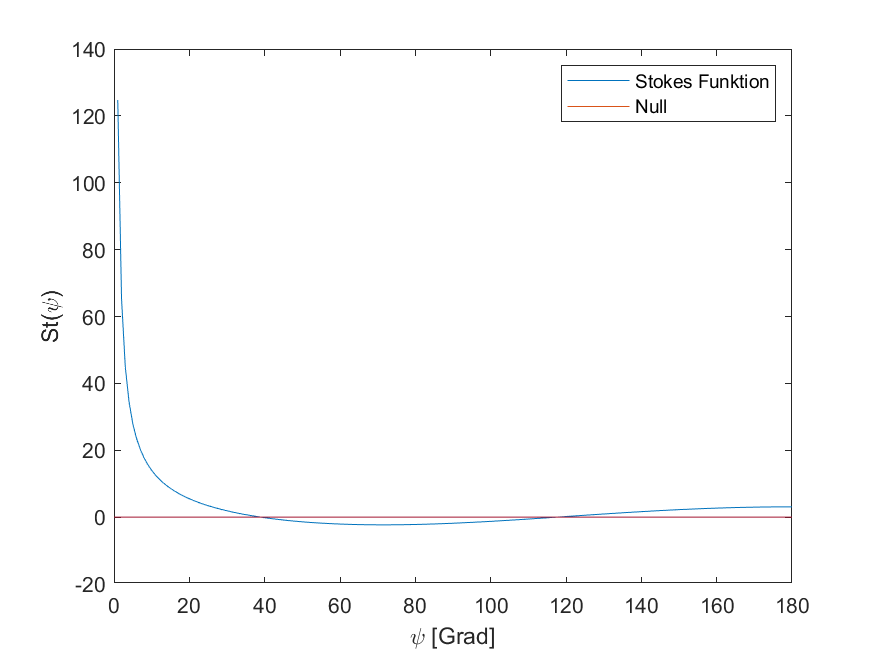
\includegraphics[scale=0.7]{stokes.png}
\caption{Visualisierung der Stokes Funktion, sowie $y=0$}
\label{stfkt}
\end{figure}

Berechnung der Nullstellen: 

\begin{gather*}
\dfrac{1}{\sin \dfrac{\psi}{2}} - 6 \sin \dfrac{\psi}{2} + 1 - 5 \cos \psi - 3 \cos \psi \cdot \ln \left(\sin \dfrac{\psi}{2} + \sin^2 \dfrac{\psi}{2}\right) = 0 \\ 
\rightarrow \psi_1 = 38.9621^{\circ} ~~~ \text{und} ~~~ \psi_2 = 117.6615^{\circ}
\end{gather*}

Angabe in Grad, Minuten, Sekunden: 

\begin{gather*}
\psi_1 = 38^{\circ} ~57' ~43'' ~~~ \text{und} ~~~ \psi_1 = 117^{\circ} ~39' ~41''
\end{gather*}

\item Berechnung der Geoidhöhen

Für die drei Punkte $P_1(48.40067893^{\circ},9.97228199^{\circ})$, $P_2(48.70311236^{\circ},9.65402314^{\circ})$ und $P_3(48.80556353^{\circ},9.21339955^{\circ})$ sollen die Geoidhöhen durch eine numerische Approximation der Integralformel von Stokes berechnet werden. Diese lautet: 

\begin{gather*}
N = \dfrac{R}{4 \pi \gamma} \iint\limits_\sigma St(\psi(\lambda_P,\varphi_P,\lambda_Q,\varphi_Q))\Delta g (\lambda_Q,\varphi_Q) d\sigma_Q 
\end{gather*}

Die berechneten Geoidhöhen lauten: 

\begin{gather*}
N_1 = 51.1588~m, ~~~ N_2 = 49.9244~m, ~~~ N_3 = 49.5306~m
\end{gather*}

\item Diskussion

Der Grund weshalb die Berechnung in Aufgabe 2b) nicht für moderne Geoidmodelle verwendet wird ist, dass die $(\lambda \times \varphi)$-Blöcke nicht als konstant angenommen werden dürfen. 

\end{enumerate}

